
By the metrics of wide adoption and industrial deployment, serializable transactions have failed. Despite the convenience and power of serializability, in today's RDBMSs, weak isolation guarantees like Read Committed isolation are overwhelmingly the default option and are sometimes the strongest (particularly among ``NewSQL'' stores)~\cite{hat-vldb}. Even within the database community, many of us have acquiesced by settling for models like Snapshot Isolation that are apparently ``good enough'' despite exposing highly nuanced Write Skew anomalies (i.e., races)~\cite{adya-isolation}. Despite the hype surrounding the return of serializability in systems like HStore~\cite{hstore}, VoltDB, and Spanner~\cite{spanner}, serializable transactions remain prohibitively expensive in a distributed (and, especially, geo-replicated) environment. (Read-only and single-partition transactions are an exception, but, as Stonebraker noted in 1985, these workloads have long been considered ``delightful'' from a concurrency control standpoint~\cite{stonebraker1985case}.) These costs are no surprise. The algorithmic forebears of these new systems~\cite{liskov-clocks,whitney-hpts,garcia-mm} pre-date the era of large-scale Internet services, and, more fundamentally, the performance, availability, and latency limitations (i.e., the \textit{coordination} overheads) are fundamental to these strong semantics rather than the faults of any given implementation~\cite{coord-avoid}. Any claims of unilateral performance or availability parity between serializable systems and weaker alternatives should be examined with suspicion.

Unfortunately, in the words of one anonymous five-star wizard of data management, ``once you give up serializability, you fall off a cliff.'' How do we program these weak isolation levels? Overwhelmingly, and, in stark contrast to the beautiful abstraction of serializability, the alternatives offered by weak isolation have been driven by studying \textit{mechanisms} rather than application requirements. For example, in 1975, faced with the observation that strict two-phase locking can be expensive, Jim Gray et al. asked~\cite{gray-isolation}: what happens if we hold read locks for shorter? A simple tweak to the locking mechanism became a new policy (Read Committed isolation) that has haunted database users for the last 38 years. When is Read Committed isolation safe for a given application? The literature lends few clues~\cite{bernstein-semantic}, and I challenge any self-respecting concurrency control researcher---or, better, the end-users we serve as a community---to provide a good answer. In retrospect, a better question might have been: what alternatives to serializability can we provide that make programming easier for developers? The former pattern of discourse dominates the exhausting literature of alternative isolation levels~\cite{hat-vldb}, some of which this author is complicit in inventing. I am hardly the first to pose the latter question, but, today, most of these alternatives lie deep in the bowels of 1980s-era concurrency control literature, largely forgotten in this new era of cloud-enabled, Big Data, web-scale data management systems.

It is high time that concurrency control systems---as deployed in practice and not simply in our undergraduate textbooks---actually serve the requirements of end-user applications. High performance non-serializable concurrency control must integrate application-level criteria as a basis for correct execution. At SIGMOD 1979, Kung and Papadimitriou taught us the (seldom heeded) lesson that, without any knowledge of application semantics, we cannot do better than serializability while ensuring correctness~\cite{kung1979optimality}. Yet the demand for more scalable, less coordination-intensive and therefore non-serializable concurrency control necessitates a shift beyond the read-write interface and towards increased application semantics.

Invariants, or declarative constraints on acceptable database states, are a promising means of capturing correctness criteria. First, invariants allow users to reason about their applications instead of low-level read/write behavior. This eliminates the error-prone process of manually translating between low-level read/write traces (i.e., prohibited phenomena that define weak isolation levels) and application correctness criteria~\cite{consistency-borders}. Second, from an implementation perspective, instead of specifying \textit{how} an application's correctness should be guaranteed, an invariant leaves considerable leeway in terms of implementation and optimization. In recent work, we have demonstrated how invariants directly determine the potential for coordination-free execution, illustrated via a 25-fold improvement in compliant TPC-C New-Order throughput and order-of-magnitude improvements over serializable isolation due to decreased coordination between concurrent transactions~\cite{coord-avoid}. Third, invariants have already crept into data management solutions in various forms, including primary key, foreign key, and check constraints. In an ongoing survey of open-source ORM-backed web applications, we have found widespread adoption of user-level invariant-based concurrency control mechanisms (e.g., Ruby on Rails Validations), which are largely undocumented in the database systems community yet, by usage, are over an order of magnitude more prevalent than transactions. The basic concept of (and arguments for) invariant-based concurrency control date to at least the early 1970s~\cite{florentin-constraints}. However, the recent rise (and re-discovery) of its similarly vintage cousins weak isolation~\cite{gray-isolation}, eventual consistency~\cite{ec-rfc}, and distributed transactions~\cite{chu-avoiding} heralds the possibility of a profitable rebirth.

Invariant-based concurrency control presents several opportunities for the CIDR community. My collaborators and I have already begun classifying common invariants as requiring coordination or not (and therefore achievable in a scalable system), yielding results as above~\cite{coord-avoid}. However, there are a range of existing challenges: how should an invariant requiring coordination actually be maintained? What is the space of programs that pass the necessary invariant confluence condition~\cite{coord-avoid}, and how should we analyze full programs beyond SQL? Which practical invariants---beyond those found in RDBMSs today---are common cases ripe for optimization~\cite{ramp-txns}? The answers to these questions, coupled with the further development of invariant-based concurrency control systems offers great promise. We can do better, and our users deserve more humane and more usable high performance database concurrency control abstractions.\vspace{-2 em}



%\begin{center}\textit{When BASE jumping off cliffs, bring a parachute.}\hspace{.25em} \raisebox{-1.3em}{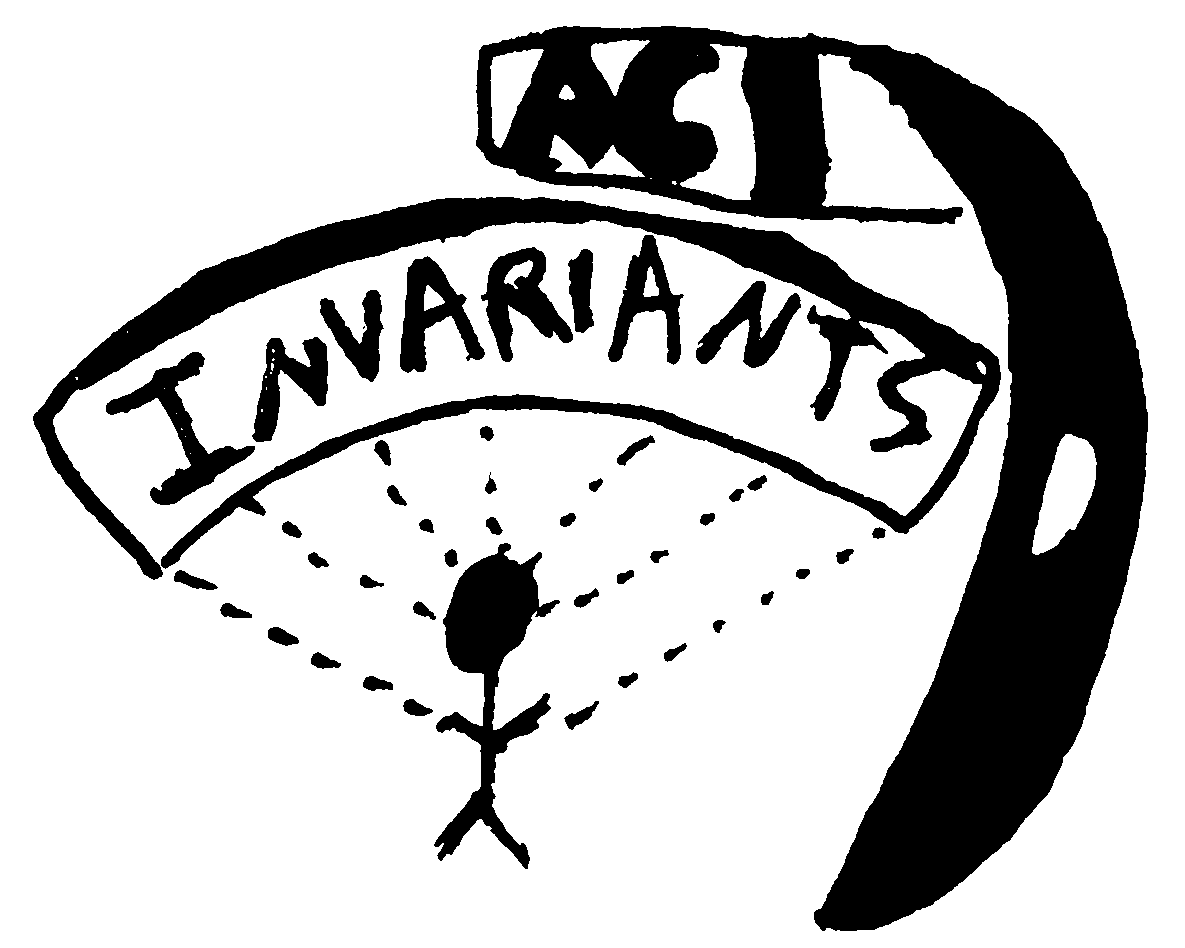
\includegraphics[width=4.5em]{parachute.png}}\end{center}


\begin{comment}


\noindent\textbf{Abstract.} \textit{Weakly consistent systems surface a controversial tension between, on the one hand, availability, latency, and performance, and, on the other, programmability. We propose the concept of coordination avoidance as a unifying, underlying principle behind the former and discuss lessons from our recent experiences mitigating the latter.}

\minihead{Trouble in paradise} Faced with the task of operating ``always on'' services and lacking sufficient guidance from the literature regarding alternative distributed designs and algorithms, many Internet service architects and engineers throughout the 2000s discarded traditional database semantics and transactional models in favor of weaker but less principled models: eventual consistency, few if any multi-object, multi-operation (i.e., transactional) guarantees, and ad-hoc application-specific compensation---collectively, much of NoSQL~\cite{queue}. From a research perspective, this space of weaker models has proven to be a fertile area: new (or re-discovered), often esoteric, and almost always nuanced semantics present many opportunities for systems designs, optimizations, and formalism.

Unfortunately, these weaker models come with serious usability disadvantages: programmability suffers. Understanding the implications of choosing a non-serializable isolation model is a difficult task. Users of have little to no practical guidance as to how to choose an appropriate model for their applications, and understanding the differences between models effectively requires graduate-level training in distributed systems and/or database theory~\cite{consistency-borders}. Members within the internet services industry that birthed the resurgence of interest in these semantics have begun a backlash against them: one recent and prominent industrial account unequivocally states that ``designing applications to cope with concurrency anomalies in their data is...ultimately not worth the performance gains''~\cite{f1}. Statements like these (which, in our experience, enjoy some popularity among practitioners and considerable acceptance in the database community~\cite{stonebraker-blog}) suggest that, as a research community, we are either failing to communicate and demonstrate the benefits of these weak semantics, have underestimated the burden placed on programmers, or a combination of both.

\minihead{Coordination-avoidance: a fundamental theme} In tribute to the CAP Theorem~\cite{gilbert-cap} that popularized this debate, much of the dialogue around weakly consistent models concerns the availability of operations under failures. Availability is an important property, but, in our opinion, a sole focus on availability undervalues the benefits of weak semantics. Abadi successfully argues that, while ``availability'' is only relevant in the presence of failures, weakly consistent (``AP'') systems can also offer low latency~\cite{pacelc}. We would take Abadi's position even further: weak consistency also allows aggressive scale-out, even at the level of a single data item---more servers can be added without communication between them. Indeed, modern, strongly consistent ``NewSQL'' systems can provide horizontal scale-out using shared-nothing database replication techniques popularized in the 1980s~\cite{sharednothing}. However, especially for worst-case accesses, these systems are far from ``as scalable as NoSQL''~\cite{f1} systems offering weak isolation. In recent research, we have examined the throughput penalties associated with these ``strong'' models: in modern LAN and WAN networks, distributed serializable transactions face a worst-case bound of 1200 and 12 read-write transactions per item per second, independent of implementation strategy. Recent systems~\cite{spanner,f1} are no exception: operations over disjoint data can proceed concurrently, increasing throughput, but operations over non-disjoint data are limited by network latency.

The three properties above---availability, low latency, and scale-out---are consequences of a more fundamental principle underlying weakly consistent systems: a lack of synchronous communication, or coordination, between concurrent operations. If operations can execute coordination-free, they can run concurrently, on any available resources, without coommunication with or stalling of concurrent operations. The cost of coordination is easily and simultaneously cast in the form of (minority) unavailability, latency (minimum 1 RTT), and throughput (maximum \textasciitilde$\frac{1}{\texttt{RTT}}$). Moreover, and more importantly, the concept of coordination-free execution is portable to more system architectures: whereas traditional formulations of availability are inherently tied to physical replication, coordination-freedom is a property of the execution strategy and is independent of physical deployment or topology. For example, a system providing clients with snapshot reads can effectively act as a coordination-free ``replicated'' system even if implemented by a set of linearizable multi-versioned masters~\cite{ramp-txns}. Judicious use of weak semantics in correct application execution equates to \textit{coordination-avoidance}~\cite{coord-avoid}: the use of as little coordination as possible.

\minihead{Bridging the gap} As F1's authors highlight above~\cite{f1}, the decision to consider coordination-avoiding algorithms or not requires a cost-benefit judgment~\cite{queue}: will performance, availability, or latency benefits outweigh the cost of ascertaining whether weak models are sufficient? In a sober assessment, many applications will likely be able to (over-)pay for ``strong consistency'': single-site operations are inexpensive~\cite{sharednothing}, while improvements in datacenter networks~\cite{bobtail} lower the cost for non-geo-replicated systems. Yet, a large class of applications---for example, non-partitionable applications~\cite{tao}, applications with high mutation rates (i.e., write contention)~\cite{tpcc}, or geo-replicated applications~\cite{swift}---will not be as tolerant of extraneous coordination costs.

Identifying and serving this latter class of applications is paramount to ensuring the future adoption of coordination-avoiding algorithms. While represents a difficult task, we offer three examples from our recent research:

\begin{myitemize}
\item \textbf{ACID databases are not built using ACID transactions.} High-performance database internals are maintained using specialized, highly optimized algorithms that are carefully designed to maximize safe concurrency~\cite{gray-book} (e.g., in the case of indexing, exotic data structures like B-link trees~\cite{blink-tree}). The database designer does not use serializable access to the database data structures for at least two reasons. First, doing so would be prohibitively expensive, and, second, the expert designer does not need to: she has a well-defined specification (e.g., secondary index lookup behavior) that she can use to ensure correctness (without end-user intervention). In a distributed database system, coordination-avoiding techniques are applicable to internal data structure maintenance. As experts of both databases and fast distributed algorithms, we can ensure that the anomalies of our weakly consistent but fast algorithms do not interfere with application-level correctness; we can encapsulate the side-effects of weak semantics behind well-defined (and existing) interfaces. Our recent work on Read Atomic Multi-Partition (RAMP) transactions was developed in this context and, as motivating use cases, focuses on foreign key constraint maintenance, distributed secondary indexing, and materialized view maintenance~\cite{ramp-txns}.

\item \textbf{Applications on ACID databases (surprisingly often) do not use ACID transactions.} Traditional databases also have an equivalent of weak consistency: although they were not explicitly developed for distributed environments, databases provide a range of ``weak isolation'' models, such as Read Committed and Repeatable Read. Many ``ACID'' databases today adopt these weak isolation guarantees by default (only 3 of 18 in a survey we recently performed) and sometimes as the strongest level supported (e.g., Oracle 11G)~\cite{hat-vldb}. Existing applications deployed on these systems are necessarily either tolerant of or otherwise must for compensate for these weak semantics, hinting at opportunities for optimization. Moreover, while many of these weak semantics are achievable in a coordination-free manner, their typical \textit{implementations} are not and require expensive locking or validation protocols---a remnant of their single-node origins. We recently classified commonly-deployed isolation models as achievable via ``Highly Available Transactions'' or not~\cite{hat-vldb} and believe the further study of these applications and associated semantics can bear additional fruit.

\item \textbf{High-value, well-specified applications are ripe for optimization.} We have found success in coordination-avoiding optimization of high-value workloads. As an example, we recently combined the above RAMP transactions with our recent results on coordination-free integrity constraints to attain an order-of-magnitude improvement in performance on the challenging TPC-C OLTP benchmark~\cite{coord-avoid,tpcc}. Coincidentally, as the industry- and academic-standard benchmark for transactional performance, TPC-C is accompanied by a rigorous specification of correctness, which was instrumental in guiding our implementation strategy. We have subsequently encountered few database workloads and integrity constraints that require coordination for \textit{all} queries. The resulting challenge is two-fold: first, identify the operations that \textit{do} require coordination (ideally few or none), and second, determine an appropriate coordination-free execution plan for those that do not.  \end{myitemize}

Overall, we have found success in $i.)$ focusing on existing applications and $ii.)$ incorporating existing specifications to enable coordination-avoiding execution. Towards these goals, our ongoing research directly incorporates application-level invariants (derived from real-world application and the SQL language) for analysis under a necessary and sufficient property for coordination-free execution~\cite{coord-avoid}. The use of application-level invariants is key to safely maximizing concurrency without requiring programmer expertise in weak isolation models.

\minihead{A coordinated future} The continued success of weakly consistent systems requires a focus on utility. Delivering an understanding of exactly \textit{why} these weakly consistent semantics can provide (in a fundamental sense) greater availability, lower latency, and higher throughput is paramount; our proposed focus on \textit{coordination avoidance} is our best attempt to do so. By applying the lens of coordination avoidance to a range of existing, well-defined and ideally high-value domains, we have the opportunity to demonstrate exactly \textit{when} weak consistency is adequate and, equally importantly, when it is not. Without a full specification, language techniques~\cite{calm,blazes} and domain-specific optimizations~\cite{crdt} are helpful to programmers. However, with a full specification and increased knowledge of application semantics~\cite{coord-avoid,ramp-txns}, we can fully realize the benefits of coordination avoidance while further mitigating programmer burden.

\end{comment}